% Options for packages loaded elsewhere
% Options for packages loaded elsewhere
\PassOptionsToPackage{unicode}{hyperref}
\PassOptionsToPackage{hyphens}{url}
\PassOptionsToPackage{dvipsnames,svgnames,x11names}{xcolor}
%
\documentclass[
  12pt,
  oneside,
  a4paper,
  english,
  brazil]{abntex2}
\usepackage{xcolor}
\usepackage[top=30mm,left=30mm,right=20mm,bottom=20mm]{geometry}
\usepackage{amsmath,amssymb}
\setcounter{secnumdepth}{5}
\usepackage{iftex}
\ifPDFTeX
  \usepackage[T1]{fontenc}
  \usepackage[utf8]{inputenc}
  \usepackage{textcomp} % provide euro and other symbols
\else % if luatex or xetex
  \usepackage{unicode-math} % this also loads fontspec
  \defaultfontfeatures{Scale=MatchLowercase}
  \defaultfontfeatures[\rmfamily]{Ligatures=TeX,Scale=1}
\fi
\usepackage{lmodern}
\ifPDFTeX\else
  % xetex/luatex font selection
\fi
% Use upquote if available, for straight quotes in verbatim environments
\IfFileExists{upquote.sty}{\usepackage{upquote}}{}
\IfFileExists{microtype.sty}{% use microtype if available
  \usepackage[]{microtype}
  \UseMicrotypeSet[protrusion]{basicmath} % disable protrusion for tt fonts
}{}
\makeatletter
\@ifundefined{KOMAClassName}{% if non-KOMA class
  \IfFileExists{parskip.sty}{%
    \usepackage{parskip}
  }{% else
    \setlength{\parindent}{0pt}
    \setlength{\parskip}{6pt plus 2pt minus 1pt}}
}{% if KOMA class
  \KOMAoptions{parskip=half}}
\makeatother
% Make \paragraph and \subparagraph free-standing
\makeatletter
\ifx\paragraph\undefined\else
  \let\oldparagraph\paragraph
  \renewcommand{\paragraph}{
    \@ifstar
      \xxxParagraphStar
      \xxxParagraphNoStar
  }
  \newcommand{\xxxParagraphStar}[1]{\oldparagraph*{#1}\mbox{}}
  \newcommand{\xxxParagraphNoStar}[1]{\oldparagraph{#1}\mbox{}}
\fi
\ifx\subparagraph\undefined\else
  \let\oldsubparagraph\subparagraph
  \renewcommand{\subparagraph}{
    \@ifstar
      \xxxSubParagraphStar
      \xxxSubParagraphNoStar
  }
  \newcommand{\xxxSubParagraphStar}[1]{\oldsubparagraph*{#1}\mbox{}}
  \newcommand{\xxxSubParagraphNoStar}[1]{\oldsubparagraph{#1}\mbox{}}
\fi
\makeatother


\usepackage{longtable,booktabs,array}
\usepackage{calc} % for calculating minipage widths
% Correct order of tables after \paragraph or \subparagraph
\usepackage{etoolbox}
\makeatletter
\patchcmd\longtable{\par}{\if@noskipsec\mbox{}\fi\par}{}{}
\makeatother
% Allow footnotes in longtable head/foot
\IfFileExists{footnotehyper.sty}{\usepackage{footnotehyper}}{\usepackage{footnote}}
\makesavenoteenv{longtable}
\usepackage{graphicx}
\makeatletter
\newsavebox\pandoc@box
\newcommand*\pandocbounded[1]{% scales image to fit in text height/width
  \sbox\pandoc@box{#1}%
  \Gscale@div\@tempa{\textheight}{\dimexpr\ht\pandoc@box+\dp\pandoc@box\relax}%
  \Gscale@div\@tempb{\linewidth}{\wd\pandoc@box}%
  \ifdim\@tempb\p@<\@tempa\p@\let\@tempa\@tempb\fi% select the smaller of both
  \ifdim\@tempa\p@<\p@\scalebox{\@tempa}{\usebox\pandoc@box}%
  \else\usebox{\pandoc@box}%
  \fi%
}
% Set default figure placement to htbp
\def\fps@figure{htbp}
\makeatother


% definitions for citeproc citations
\NewDocumentCommand\citeproctext{}{}
\NewDocumentCommand\citeproc{mm}{%
  \begingroup\def\citeproctext{#2}\cite{#1}\endgroup}
\makeatletter
 % allow citations to break across lines
 \let\@cite@ofmt\@firstofone
 % avoid brackets around text for \cite:
 \def\@biblabel#1{}
 \def\@cite#1#2{{#1\if@tempswa , #2\fi}}
\makeatother
\newlength{\cslhangindent}
\setlength{\cslhangindent}{1.5em}
\newlength{\csllabelwidth}
\setlength{\csllabelwidth}{3em}
\newenvironment{CSLReferences}[2] % #1 hanging-indent, #2 entry-spacing
 {\begin{list}{}{%
  \setlength{\itemindent}{0pt}
  \setlength{\leftmargin}{0pt}
  \setlength{\parsep}{0pt}
  % turn on hanging indent if param 1 is 1
  \ifodd #1
   \setlength{\leftmargin}{\cslhangindent}
   \setlength{\itemindent}{-1\cslhangindent}
  \fi
  % set entry spacing
  \setlength{\itemsep}{#2\baselineskip}}}
 {\end{list}}
\usepackage{calc}
\newcommand{\CSLBlock}[1]{\hfill\break\parbox[t]{\linewidth}{\strut\ignorespaces#1\strut}}
\newcommand{\CSLLeftMargin}[1]{\parbox[t]{\csllabelwidth}{\strut#1\strut}}
\newcommand{\CSLRightInline}[1]{\parbox[t]{\linewidth - \csllabelwidth}{\strut#1\strut}}
\newcommand{\CSLIndent}[1]{\hspace{\cslhangindent}#1}



\setlength{\emergencystretch}{3em} % prevent overfull lines

\providecommand{\tightlist}{%
  \setlength{\itemsep}{0pt}\setlength{\parskip}{0pt}}



 


% ---
% Pacotes básicos 
% ---
\usepackage{lmodern}			% Usa a fonte Latin Modern			
\usepackage[T1]{fontenc}		% Selecao de codigos de fonte.
\usepackage[utf8]{inputenc}		% Codificacao do documento (conversão automática dos acentos)
\usepackage{lastpage}			% Usado pela Ficha catalográfica
\usepackage{indentfirst}		% Indenta o primeiro parágrafo de cada seção.
\usepackage{color}				% Controle das cores
\usepackage{graphicx}			% Inclusão de gráficos
\usepackage{microtype} 			% para melhorias de justificação
\usepackage{amsmath}
\usepackage{amssymb}
\usepackage{upgreek}
\usepackage{listings}			% Inclusão de código fonte 			


% Pacotes de citações
% ---
\usepackage[brazilian,hyperpageref]{backref}	 % Paginas com as citações na bibl
\usepackage[alf]{abntex2cite}	% Citações padrão ABNT

% --- 
% CONFIGURAÇÕES DE PACOTES
% --- 

% ---
% Configurações do pacote backref
% Usado sem a opção hyperpageref de backref
\renewcommand{\backrefpagesname}{Citado na(s) página(s):~}
% Texto padrão antes do número das páginas
\renewcommand{\backref}{}
% Define os textos da citação
\renewcommand*{\backrefalt}[4]{
	\ifcase #1 %
		Nenhuma citação no texto.%
	\or
		Citado na página #2.%
	\else
		Citado #1 vezes nas páginas #2.%
	\fi}%
% ---

% ---
% Configurações de aparência do PDF final

% alterando o aspecto da cor azul
\definecolor{blue}{RGB}{41,5,195}

% informações do PDF
\makeatletter
\hypersetup{
     	%pagebackref=true,
		% pdftitle={\@title}, 
		% pdfauthor={\@author},
    	% pdfsubject={\imprimirpreambulo},
	    % pdfcreator={LaTeX with abnTeX2},
		% pdfkeywords={abnt}{latex}{abntex}{abntex2}{trabalho acadêmico}, 
		colorlinks=true,       		% false: boxed links; true: colored links
    	linkcolor=blue,          	% color of internal links
    	citecolor=blue,        		% color of links to bibliography
    	filecolor=magenta,      		% color of file links
		urlcolor=blue,
		bookmarksdepth=4
}

% Comandos de uso do orientador para sugestão de alterações:
\usepackage{xcolor}
\usepackage{cancel}

\colorlet{oliveGreen}{blue!20!black!50!green}

\usepackage{soul}
\usepackage{soulutf8}
\setstcolor{red}

\newcommand{\cito}[1]{\textsuperscript{\cite{#1}}} % numeração da citação sobreescrita
\newcommand{\PROFESSOR}[1]{\textcolor{red}{\MakeUppercase{#1}}} % Acrescenta um nota pelo professor
\newcommand{\PROFESSORDEL}[1]{\textcolor{red}{\st{#1}}} % removido pelo professor
\newcommand{\PROFESSORADD}[1]{\textcolor{oliveGreen}{#1}} % adicionado pelo professor
\newcommand{\PROFESSORREP}[2]{\PROFESSORDEL{#1}\PROFESSORADD{#2}} % substituir


\renewcommand{\printtoctitle}[1]{\normalsize\bfseries\centering TABLE OF CONTENTS}


% Adiciona indentação para seções e subseções no sumário
\cftsetindents{chapter}{0em}{0em}
\cftsetindents{section}{1.5em}{2.5em}
\cftsetindents{subsection}{3em}{3.5em}

\AtBeginDocument{\captionsetup{labelfont=bf}}


\makeatother
% --- 

% --- 
% Espaçamentos entre linhas e parágrafos 
% --- 

% O tamanho do parágrafo é dado por:
\setlength{\parindent}{1.3cm}

% Controle do espaçamento entre um parágrafo e outro:
\setlength{\parskip}{0.2cm}  % tente também \onelineskip

% ---
% compila o indice
% ---
\makeindex
% ---
\makeatletter
\@ifpackageloaded{caption}{}{\usepackage{caption}}
\AtBeginDocument{%
\ifdefined\contentsname
  \renewcommand*\contentsname{Table of contents}
\else
  \newcommand\contentsname{Table of contents}
\fi
\ifdefined\listfigurename
  \renewcommand*\listfigurename{List of Figures}
\else
  \newcommand\listfigurename{List of Figures}
\fi
\ifdefined\listtablename
  \renewcommand*\listtablename{List of Tables}
\else
  \newcommand\listtablename{List of Tables}
\fi
\ifdefined\figurename
  \renewcommand*\figurename{Figure}
\else
  \newcommand\figurename{Figure}
\fi
\ifdefined\tablename
  \renewcommand*\tablename{Table}
\else
  \newcommand\tablename{Table}
\fi
}
\@ifpackageloaded{float}{}{\usepackage{float}}
\floatstyle{ruled}
\@ifundefined{c@chapter}{\newfloat{codelisting}{h}{lop}}{\newfloat{codelisting}{h}{lop}[chapter]}
\floatname{codelisting}{Code}
\newcommand*\listoflistings{\listof{codelisting}{List of Code}}
\makeatother
\makeatletter
\makeatother
\makeatletter
\@ifpackageloaded{caption}{}{\usepackage{caption}}
\@ifpackageloaded{subcaption}{}{\usepackage{subcaption}}
\makeatother
\makeatletter
\@ifpackageloaded{tcolorbox}{}{\usepackage[skins,breakable]{tcolorbox}}
\makeatother
\makeatletter
\@ifundefined{shadecolor}{\definecolor{shadecolor}{rgb}{.97, .97, .97}}{}
\makeatother
\makeatletter
\makeatother
\makeatletter
\ifdefined\Shaded\renewenvironment{Shaded}{\begin{tcolorbox}[interior hidden, frame hidden, borderline west={3pt}{0pt}{shadecolor}, enhanced, breakable, sharp corners, boxrule=0pt]}{\end{tcolorbox}}\fi
\makeatother
\usepackage{bookmark}
\IfFileExists{xurl.sty}{\usepackage{xurl}}{} % add URL line breaks if available
\urlstyle{same}
\hypersetup{
  colorlinks=true,
  linkcolor={blue},
  filecolor={Maroon},
  citecolor={Blue},
  urlcolor={Blue},
  pdfcreator={LaTeX via pandoc}}


\author{}
\date{}
\begin{document}


\chapter{\textbf{Materials and Methods}}

This chapter details the methodology for developing a Level 1 digital
twin for a laboratory-scale gas turbine. The approach integrates
first-principle thermodynamic models with a data-driven framework using
Physics-Informed Neural Networks (PINNs). The primary objective is to
create a robust and physically consistent model capable of predicting
the turbine's performance under various operating conditions. The
methodology encompasses several key stages: establishing the
mathematical model from fundamental thermodynamic laws, leveraging
experimental data for training and validation, implementing the hybrid
PINN architecture, and rigorously evaluating the final digital twin's
predictive accuracy and physical fidelity. This structured approach
ensures that the resulting digital twin is not only accurate but also
grounded in the underlying physics of the gas turbine system.

\section{Experimental Setup and Data
Acquisition}\label{experimental-setup-and-data-acquisition}

The physical asset central to this investigation is the Mini-Lab Gas
Turbine Power System, which is based on the SR-30 turbojet engine. This
system is purpose-built for educational and experimental applications,
allowing for the simulation and detailed analysis of core gas turbine
operations and thermodynamic cycles on a laboratory scale.

\subsection{System Overview and
Instrumentation}\label{system-overview-and-instrumentation}

The SR-30 engine is configured as a single-shaft turbojet, comprising a
centrifugal compressor, an annular combustion chamber, an axial turbine,
and a nozzle. To facilitate comprehensive operational monitoring and
data acquisition, the engine is extensively instrumented with a variety
of sensors. These sensors provide high-resolution, real-time data on
critical thermodynamic and performance parameters.

The instrumentation setup includes:

\begin{itemize}
    \item Compressor Inlet Pressure ($\mathrm{P}_{1}$) and Temperature ($\mathrm{T}_{1}$).
    \item Compressor Exit Pressure ($\mathrm{P}_{2}$) and Temperature ($\mathrm{T}_{2}$).
    \item Turbine Inlet Pressure ($\mathrm{P}_{3}$) and Temperature ($\mathrm{T}_{3}$).
    \item Turbine Exit Pressure ($\mathrm{P}_{4}$) and Temperature ($\mathrm{T}_{4}$).
    \item Exhaust Gas Pressure ($\mathrm{P}_{5}$) and Temperature ($\mathrm{T}_{5}$).
    \item Compressor Rotational Speed (RPM), measured by a tachometer generator.
    \item Fuel Pressure and Fuel Flow.
    \item Engine Thrust, measured via a dedicated load cell.
\end{itemize}

These parameters are displayed on the system's control panel and, more
extensively, on a connected Data Acquisition Screen. Specifically,
\(\mathrm{P}_{3}\) and \(\mathrm{T}_{3}\) (Turbine Inlet Temperature,
displayed as TIT) are available on both the panel and screen, while
\(\mathrm{T}_{5}\) (Exhaust Gas Temperature, displayed as EGT) is also
accessible from both. Fuel Pressure is displayed on the panel. The
precise location of these engine sensors is depicted in the SR-30 Gas
Turbine Cutaway diagram within the Mini-Lab's operational manual.

\begin{figure}

\caption{\label{fig-turbine-schema}Schematic of Brayton Cycle for Gas
Turbine and Cut Away of SR-30 Engine.}

\begin{minipage}{\linewidth}
\pandocbounded{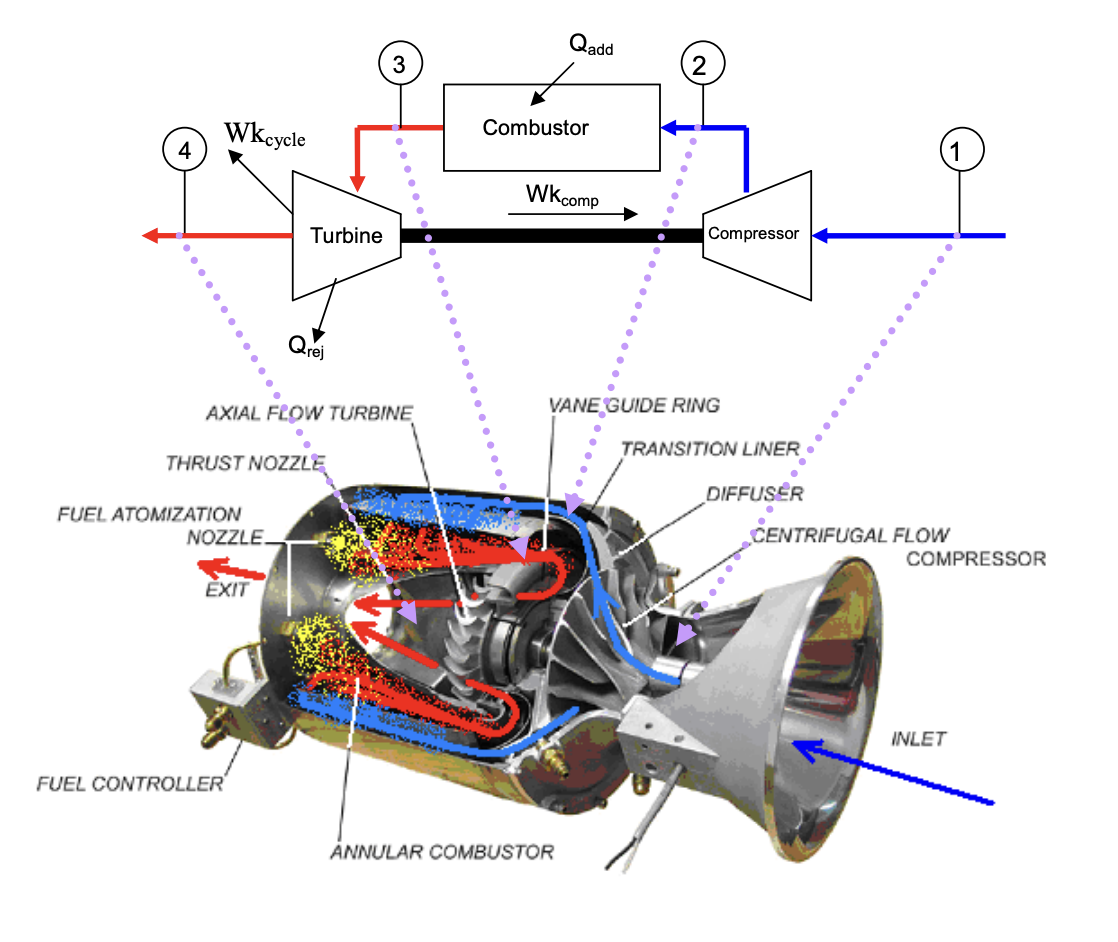
\includegraphics[keepaspectratio]{figuras/turbine_schema.png}}\end{minipage}%
\newline
\begin{minipage}{\linewidth}
Source: Mini-Lab Gas Turbine Power System Manual Turbine Technologies,
Ltd.
(\citeproc{ref-TurbineTechnologies2011MiniLab}{2011})\end{minipage}%

\end{figure}%

\subsection{Data Acquisition System and Control
Interface}\label{data-acquisition-system-and-control-interface}

The data acquisition process is managed through a dedicated Data
Acquisition Computer running the MiniLab 1.1 software. This computer
connects to the Mini-Lab system via a USB port, leveraging a National
Instruments DAQ (Data Acquisition) system (specifically the NI DAQ 6218
module) for real-time data capture and display. The MiniLab 1.1 software
facilitates logging data to file, displaying plot features, and offers
controls for unit toggling (e.g., Celsius to Fahrenheit for
temperatures, Psig to kPa for pressures, Liters/hour or Gallons/hour for
fuel flow, and Newtons to Pounds for thrust). The data sampling rate can
be selected between 0.1 and 5 samples per second.

\subsection{Experimental Procedure and Data Collection
Protocol}\label{experimental-procedure-and-data-collection-protocol}

The experimental procedure involved operating the Mini-Lab gas turbine
through its pre-start, start-up, and operational phases, followed by a
controlled shutdown. Prior to each run, essential checks were conducted,
including verification of fuel properties and ambient barometric
pressure \(P_{amb}=946.7 mbar\). During operation, the MiniLab 1.1
software collected real-time data from various sensors, including
temperatures, pressures, fuel flow, RPM, and thrust. This data was
logged continuously to a file on the connected computer's hard drive via
a USB connection to a National Instruments DAQ system. The software
allowed for adjustable sampling rates, and the recorded data was stored
in an ASCII format, enabling direct import into spreadsheet programs for
subsequent detailed analysis.

\section{Thermodynamic Modeling of the Gas Turbine
System}\label{thermodynamic-modeling-of-the-gas-turbine-system}

\subsection{System Overview}\label{system-overview}

The system of interest is a small-scale gas turbine engine operating in
steady-state. It consists of the following major components:

\begin{itemize}
    \item Compressor: Increases the pressure and temperature of incoming ambient air.
    \item Combustor: Mixes compressed air with fuel, where combustion raises the temperature significantly.
    \item Turbine: Extracts energy from the hot combustion gases to drive the compressor and generate useful work.
    \item Nozzle (Exhaust Section): Accelerates the exhaust gases to produce thrust.
\end{itemize}

Each component operates under the assumption of quasi-one-dimensional,
steady, adiabatic flow, with negligible heat loss to the surroundings
unless explicitly modeled.

\subsection{Assumptions and
Idealizations}\label{assumptions-and-idealizations}

To derive tractable analytical expressions and guide neural network
constraints, the following assumptions are adopted:

\begin{itemize}
    \item The working fluid (air and combustion gases) behaves as a calorically perfect ideal gas:
$$
    P = \rho R T, \quad c_p, c_v \text{ constant}, \quad \gamma = \frac{c_p}{c_v} \approx 1.4
$$

    \item Isentropic relations apply to ideal compression and expansion processes with specified efficiencies $\eta_c$ (compressor) and $\eta_t$ (turbine).
    \item Constant specific heats $c_p$ and $c_v$ are used, consistent with the assumption of ideal gases.
    \item No heat transfer or pressure losses in ducts, except where captured by model residuals.
    \item Steady-state and quasi-1D flow are assumed throughout.
\end{itemize}

\subsection{Key Thermodynamic
Equations}\label{key-thermodynamic-equations}

\subsubsection{Compressor}\label{compressor}

\begin{itemize}
    \item Isentropic temperature relation:
$$
    \frac{T_{2s}}{T_1} = \left( \frac{P_2}{P_1} \right)^{\frac{\gamma - 1}{\gamma}}
$$

    \item Actual outlet temperature considering efficiency:
$$
    T_2 = T_1 + \frac{T_{2s} - T_1}{\eta_c}
$$

    \item Power required by the compressor:
$$
    W_{\text{comp}} = \dot{m}_a c_p (T_2 - T_1)
$$

\end{itemize}

\subsubsection{Combustor}\label{combustor}

\begin{itemize}
    \item Energy balance (idealized with complete combustion and no heat losses):
$$
    \dot{m}_f Q_{\text{HV}} = (\dot{m}_a + \dot{m}_f) c_p (T_3 - T_2)
$$

    where $Q_{\text{HV}}$ is the lower heating value of the fuel and the gas mass flow is $\dot{m}_g = \dot{m}_a + \dot{m}_f$.
\end{itemize}

\subsubsection{Turbine}\label{turbine}

\begin{itemize}
    \item Isentropic temperature relation:
$$
    \frac{T_{4s}}{T_3} = \left( \frac{P_4}{P_3} \right)^{\frac{\gamma - 1}{\gamma}}
$$

    \item Actual outlet temperature considering turbine efficiency:
$$
    T_4 = T_3 - \eta_t (T_3 - T_{4s})
$$

    \item Power generated by the turbine:
$$
    W_{\text{turb}} = (\dot{m}_a + \dot{m}_f) c_p (T_3 - T_4)
$$

\end{itemize}

\subsubsection{Nozzle (Exhaust)}\label{nozzle-exhaust}

Assuming isentropic expansion and ambient back pressure \(P_0\), the
exhaust velocity is: \[
V_{\text{exit}} = \sqrt{2 c_p T_5 \left( 1 - \left( \frac{P_0}{P_5} \right)^{\frac{\gamma - 1}{\gamma}} \right)}
\]

The thrust is then calculated via momentum balance: \[
F = (\dot{m}_a + \dot{m}_f) (V_{\text{exit}} - V_{\text{inlet}})
\]

If inlet velocity is negligible (static tests), this simplifies to: \[
F \approx (\dot{m}_a + \dot{m}_f) V_{\text{exit}}
\]

\subsection{Station Numbering
Convention}\label{station-numbering-convention}

To standardize variables across the PINN and thermodynamic sections:

\begin{center}
\begin{tabular}{ll}
$1$ & Ambient conditions (inlet to compressor) \\
$2$ & Compressor exit / combustor inlet \\
$3$ & Combustor exit / turbine inlet \\
$4$ & Turbine exit / nozzle inlet \\
$5$ & Nozzle exit (exhaust gas temperature station)
\end{tabular}
\end{center}

This convention allows the PINN to learn both the observable outputs
(\(T_3\), \(T_5\), \(F\)) and intermediate station states (\(T_2\),
\(P_2\), \(T_4\), \(P_4\), etc.), constrained by physics-based
residuals.

\section{Physics-Informed Neural Network (PINN)
Framework}\label{physics-informed-neural-network-pinn-framework}

To bridge the gap between purely data-driven models and first-principle
simulations, this work employs a Physics-Informed Neural Network (PINN)
to model the gas turbine system.

\subsection{Core Concept}\label{core-concept}

PINNs are neural networks that embed physical laws directly into their
training process. Rather than minimizing only the error between model
predictions and experimental data, the PINN loss function also includes
terms that penalize violations of governing physical equations. This
approach ensures that predictions are both data-accurate and physically
consistent, even in regions where data is sparse.

\subsection{PINN Architecture}\label{pinn-architecture}

The core model is a fully connected Multi-Layer Perceptron (MLP) trained
to learn mappings from inputs to thermodynamic states and performance
metrics. The architecture is guided by simplifying assumptions from
thermodynamics:

\begin{itemize}
    \item Air is modeled as a calorically perfect ideal gas with constant specific heats ($c_p$, $c_v$) and a constant heat capacity ratio $\gamma = c_p / c_v \approx 1.4$.
    \item Isentropic efficiencies for the compressor ($\eta_c$) and turbine ($\eta_t$) are assumed constant.
    \item Heat losses, frictional effects, and pressure drops outside of defined station points are neglected.
\end{itemize}

Inputs: Key operational parameters that determine the thermodynamic
state of the system:

\begin{itemize}
    \item Fuel flow rate $\dot{m}_f$ ($\mathrm{kg/s}$)
    \item Compressor rotational speed $N_1$ (RPM)
    \item Ambient temperature $T_1$ (K)
    \item Ambient pressure $P_1$ (Pa)
\end{itemize}

Outputs: Predicted thermodynamic variables and performance indicators:

\begin{itemize}
    \item Station states: $T_{2,\text{pred}}, P_{2,\text{pred}}, T_{3,\text{pred}}, P_{3,\text{pred}}, T_{4,\text{pred}}, P_{4,\text{pred}}, T_{5,\text{pred}}, P_{5,\text{pred}}$
    \item Net thrust $F_{\text{pred}}$ (N)
\end{itemize}

\subsection{Hybrid Loss Function}\label{hybrid-loss-function}

The total loss used to train the PINN is a weighted sum of data-driven
and physics-based components: \[
L_{\text{total}} = w_{\text{data}} L_{\text{data}} + w_{\text{physics}} L_{\text{physics}}
\]

\begin{itemize}
    \item Data Loss ($L_{\text{data}}$): A supervised learning loss (Mean Squared Error) that penalizes deviation from available experimental measurements:
$$
    L_{\text{data}} = \frac{1}{N} \sum_{i=1}^{N} \left( y_i - y_{i,\text{pred}} \right)^2
$$
    
    \item Physics Loss ($L_{\text{physics}}$): A sum of residuals derived from physical principles, each enforcing thermodynamic consistency.
\end{itemize}

\subsubsection{\texorpdfstring{Compressor Temperature Rise Loss
(\(L_{T2}\))}{Compressor Temperature Rise Loss (L\_\{T2\})}}\label{compressor-temperature-rise-loss-l_t2}

Derived from the isentropic temperature relation: \[
L_{T2} = \left( \eta_c (T_{2,\text{pred}} - T_1) - T_1 \left( \left(\frac{P_{2,\text{pred}}}{P_1}\right)^{\frac{\gamma-1}{\gamma}} - 1 \right) \right)^2
\]

\subsubsection{\texorpdfstring{Turbine Temperature Drop Loss
(\(L_{T4}\))}{Turbine Temperature Drop Loss (L\_\{T4\})}}\label{turbine-temperature-drop-loss-l_t4}

Enforcing the relationship between pressure drop and temperature drop
across the turbine: \[
L_{T4} = \left( (T_{3,\text{pred}} - T_{4,\text{pred}}) - \eta_t T_{3,\text{pred}} \left(1 - \left(\frac{P_{4,\text{pred}}}{P_{3,\text{pred}}}\right)^{\frac{\gamma-1}{\gamma}}\right) \right)^2
\]

\subsubsection{\texorpdfstring{Shaft Power Balance Loss
(\(L_{\text{power}}\))}{Shaft Power Balance Loss (L\_\{\textbackslash text\{power\}\})}}\label{shaft-power-balance-loss-l_textpower}

For a single-shaft turbojet, the power generated by the turbine
(\(W_{\text{turb}}\)) is consumed entirely by the compressor
(\(W_{\text{comp}}\)). This constraint,
\(W_{\text{turb}} = W_{\text{comp}}\), provides a fundamental physical
link between the component states. The loss residual enforces this
balance. \[
L_{\text{power}} = \left( (\dot{m}_a + \dot{m}_f) c_p (T_{3,\text{pred}} - T_{4,\text{pred}}) - \dot{m}_a c_p (T_{2,\text{pred}} - T_1) \right)^2
\]

\subsubsection{\texorpdfstring{Combustor Energy Balance Loss
(\(L_{\text{comb}}\))}{Combustor Energy Balance Loss (L\_\{\textbackslash text\{comb\}\})}}\label{combustor-energy-balance-loss-l_textcomb}

Assuming ideal heat release with no losses: \[
L_{\text{comb}} = \left( \dot{m}_f Q_{\text{HV}} - (\dot{m}_a + \dot{m}_f) c_p (T_{3,\text{pred}} - T_{2,\text{pred}}) \right)^2
\]

\subsubsection{Thrust Loss}\label{thrust-loss}

A simplified thrust estimation (using momentum conservation) could also
be encoded if exit velocity and intake velocity are known or modeled: \[
L_{\text{thrust}} = \left( F_{\text{pred}} - (\dot{m}_a + \dot{m}_f) (V_{\text{exit}}) \right)^2
\]

Where the air mass flow \(\dot{m}_a\) can either be estimated from
\(N_1\) and ambient conditions or treated as a learnable parameter.

\section{Digital Twin Development and
Evaluation}\label{digital-twin-development-and-evaluation}

\subsection{Problem Definition}\label{problem-definition}

The primary goal of this thesis is to build a digital twin capable of
predicting steady-state thrust, combustor outlet temperature
(\(T_{3,\text{pred}}\)), and exhaust gas temperature
(\(T_{5,\text{pred}}\)) based on operational inputs: fuel flow rate and
compressor speed (\(N_1\)). Intermediate variables---such as
\(T_{2,\text{pred}}\), \(P_{2,\text{pred}}\), \(T_{4,\text{pred}}\),
\(P_{4,\text{pred}}\), \(P_{3,\text{pred}}\), and
\(P_{5,\text{pred}}\)---are also predicted to ensure thermodynamic
consistency via physics-informed residual losses.

\subsection{Data Preparation and
Preprocessing}\label{data-preparation-and-preprocessing}

The experimental dataset is preprocessed as follows:

\begin{itemize}
    \item Cleaning: Missing values are handled, and outliers are identified and removed.
    \item Unit Conversion: All quantities are converted to SI units (e.g., temperatures in Kelvin, pressures in Pascals, fuel flow in $\mathrm{kg/s}$).
    \item Normalization: Input and output features are scaled (e.g., to $[0, 1]$) to improve training stability.
    \item Data Splitting: The dataset is split into training, validation, and test sets for unbiased evaluation.
\end{itemize}

\subsection{Training and Validation}\label{training-and-validation}

The PINN is trained using gradient-based optimizers (e.g., Adam and
L-BFGS), enabled by automatic differentiation frameworks (e.g., PyTorch,
TensorFlow). Evaluation of model performance involves three key
dimensions:

\begin{itemize}
    \item Predictive Accuracy: Assessed via Mean Squared Error (MSE) and $R^2$ score on test data.
    \item Physical Consistency: Measured by evaluating the magnitude of physics loss terms across the test set.
    \item Sensitivity Analysis: Conducted to examine how predictions respond to variations in fuel flow and compressor speed, and to identify dominant factors influencing performance.
\end{itemize}

This iterative cycle of training, validation, and physics-based
refinement continues until the model achieves both data accuracy and
alignment with physical laws.

\phantomsection\label{refs}
\begin{CSLReferences}{1}{0}
\bibitem[\citeproctext]{ref-TurbineTechnologies2011MiniLab}
Turbine Technologies, Ltd. 2011. \emph{Mini-Lab Gas Turbine Power
System{\texttrademark} Sample Lab Experiment Manual}. Turbine
Technologies, Ltd.

\end{CSLReferences}




\end{document}
